% Hopefully this will be the final version of Problem statement.
This chapter introduces this research proposal. it starts with the problem statement, then outlines the motivations, research goals and the organisation of this proposal.

\section{Problem statement}

% \bx{what is cloud computing and why it is the pillar of software and other related industry. (importance of cloud computing.)}
% \bx{
% \begin{itemize}
% 	\item (what) the main challenge for cloud provider is to reduce energy consumption
% 	\item why it is important and so what? (consequences?),
% 	\item how to deal with it? (technologies)
% \end{itemize}}
\bx{Cloud computing has made a huge impact on modern software industry by offering on-demand computing capacity (e.g storage and  computing) over the internet \cite{2010arxiv1006.0308b}}. With no upfront investment, low price, and high availability (e.g services are accessible 99.99\% of the time), most web service providers such as google and neflix deploy their services (e.g. google drive) on cloud \cite{adhikari:2012uq}. 

\bx{A major issue in cloud computing is the huge energy consumption generated by data centers} - a typical data center consumes as much energy as 25,000 households \cite{dayarathna:2016ua}. Huge energy consumption has become the major expense of cloud providers. The reduction of energy bill will further beneficial to the software industry as well as most people who access the Internet on a daily basis.

\bx{To reduce the energy consumption of a data center, the main target is to reduce the number of live physical machines (PMs) (e.g. servers).} In a data center, the energy consumption can be derived from cooling system, PMs, and network devices. Currently, huge energy reduction can be achieved from PMs, because they accounts for the majority - more than 40\% - of energy consumption. PMs often run in a low utilization, e.g. from 10\% to 50\% of required resources on average because of the defects in resource management \cite{Barroso:2007jt, Shen:2015hm}. Therefore, it is possible to reduce energy by improving the utilization of PMs.
% This is because cloud users tend to preserve more resources in order to guarantee the performance when facing the variation of workloads.

\bx{The common way to reduce the energy consumption of a data center is through resource management of PMs \cite{Manvi:2014hm} (see Figure \ref{fig:workflow}).} In general, cloud resource management is a centralized system \cite{Jennings:2015ht} that allocates resources such as CPUs and memories to cloud users' applications, handles the workload fluctuations. Better management of application placement and workloads leads to the reduction of energy. 

\bx{Among four steps in resource management (see Figure \ref{fig:workflow}), \emph{server consolidation} has a crucial influence on reducing the energy consumption}. Placement decision determines the location of applications based on applications' resource requirement provided by the second resource management step - resource analysis. The decision relies on an optimization process called server consolidation which decides the placement of applications for the best energy efficiency. 
\begin{figure}
	\centering
	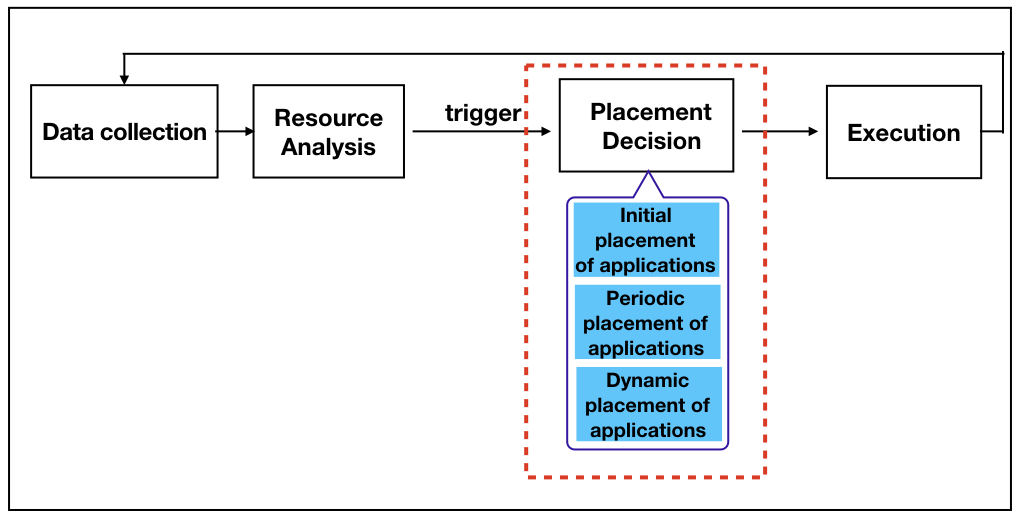
\includegraphics[width=0.7\textwidth]{pics/workflow_management.png}
	\caption{A workflow of resource management \cite{Mishra:2012kx}}
	\label{fig:workflow}
\end{figure}

% Data collection gathers resource utilization information from individual PMs and VMs such as CPU, memory utilization in a period of time. These data are collected by monitoring softwares for data analysis. Data analysis takes the collected data as the input, cleans and analyzes them. It outputs the quantity of demand resources of applications. Finally, execution places the applications to the target PMs. 

% \bx{Among these resource management steps, placement decision is the crucial step which includes three scenarios: application initial placement, periodic optimization and overloading & under-loading adjustment.} Essentially, these three scenarios contain a common strategy called server consolidation.

\bx{Server consolidation \cite{Varasteh:2015fu} is an approach to efficiently use the resources of PMs in order to reduce the total number of PMs which leads to lower energy consumption.} For three resource management scenarios, server consolidation is applied in two different ways: static and dynamic. Static approach is conducted in an off-line fashion which includes application initial placement and periodic optimization, while dynamic approach is conducted in an on-line fashion: over-loading and under-loading scenarios are in this category.


\bx{Currently, resource management in data centers is based on \emph{virtualization} technology\cite{Uhlig:2005do}. } Such virtualization separates the resources (e.g. CPUs and RAMs) of a PM into several parts called \emph{virtual machines (VMs)}, each of which runs an isolated operating system. Before virtualization technology was widely used, a traditional data center assigns a PM for each application; it leads to the low reserved utilization of PMs. To improve the resource utilization, the technique of VM is introduced. Applications are allocated to VMs which are belong to different PMs. The utilization of PMs has been largely improved and energy consumption are reduced. 

\bx{However, in recent years, resource management with VMs cannot catch up with a new trend in software industry - Service Oriented Architecture (SOA) \cite{Sprott:2004wt};} SOA has become widely used in modern software industry because of its agility and re-usability \cite{Sprott:2004wt}. SOA separates a centralized application into multiple distributed components called web services. As most of web services only require a small amount of resources,  using a VM for a web service causes resource wastage inside a VM. Consequently the low utilization of PMs decreases the energy efficiency. 


\bx{To further improve the resource of PMs and reduce energy consumption. A new virtualization technology: containers \cite{Felter:2015ki, Soltesz:2007cu} has been proposed to provide a finer granularity level of resource management.} A container is an operating system (OS) level of virtualization which run on top of VMs. A container provides performance and resource isolation for a single application so that multiple applications can run in the same VM without interfering each other. In addition, containers naturally support vertical scaling (change its size during runtime)\cite{Vaquero:2011gb} which is resilient to the fluctuate workloads.  
% CaaS uses containers as the fundamental resource management units. Thus, CaaS has the potential to improve the energy efficiency \cite{Esposito:2016br}. 

\bz{Container is still a new technology which brings new challenges in server consolidation.} Current server consolidation algorithms cannot be directly applied on container-based server consolidation problem. We will discuss the motivations in terms of three placement decision scenarios: application initial placement, periodic optimization, and dynamic placement.

% In summary, in order to improve energy efficiency in container-based data center, this research aims at proposing new models and algorithms for three placement decision scenarios:application initial placement, periodic optimization, and dynamic placement. In the following section, we will discuss the challenges in these scenarios.

% \bx{Despite which virtualization is used, server consolidation can be applied in three resource management scenarios:} application initial placement  \cite{Jennings:2015ht}, periodic optimization \cite{Mishra:2012kx} and overloading/under-loading adjustments \cite{Mishra:2012kx} (see Figure \ref{fig:workflow}).

 % Server consumption is essentially an optimization task where it adjusts applications' locations in PMs so that a minimum number of PMs is used. For a certain number of applications, the fewer number of PMs is used, the less energy is consumed. 

% Three management processes: application initial placement, periodic optimization ,   have distinct characteristics, hence, the server consolidation techniques applied on them can be roughly classified into two categories: static \cite{Xiao:2015ik} and dynamic \cite{Beloglazov:2012bw}.

% \bx{In Initial application placement, the consolidation can be described as a static task conducted in an off-line manner.} 
\vspace{5mm}
